 \section{Method}\label{methodology}
This section describes the methodology of the paper. First, in Section \ref{model}, the optimization model used is explained in detail. The focus is thereby on the mathematical formulation. However, where meaningful, qualitative explanations (i.e., supplement to the mathematical formulation) are added to give the reader a more complete understanding of the model. These qualitative explanations are used in particular to describe the main decision made by the model between maintaining operation, decommissioning or making replacement investment in existing gas grid pipelines. In Section \ref{gas_grid_austria}, the gas grid in Austria, which serves as the case study in this paper is presented. Finally, in Section \ref{scenarios}, the four different scenarios are shown.\footnote{To help the reader, the following should be noted briefly. Large parts of this paper can also be found in the comprehensive report "Role of the gas infrastrucutre in a climate-neutral Austria" (original title in German language: \textit{Rolle der Gasinfrastruktur in einem klimaneutralen Österreich}) published by the Federal Ministry Republic of Republic Austria for Climate Action, Environment, Energy, Mobility, Innovation and Technology \cite{frontier2023}. The authors of the paper here are the main authors of the full report. Against this background, the paper here is an attempt to publish the quintessence of this report and thus make it available, in particular, to the scientific community. This is explicitly mentioned here because the authors are aware that the text in this paper is deliberately kept rather short at some points in the methods section, for example in the description of the scenarios. If necessary, the full report can be consulted for additional information.}

 \subsection{Optimization model}\label{model}
 
The optimization model used, which is an optimal solution finding the economic trade-off between the capital and operating costs of the grid (mainly pipeline costs) and the revenues for meeting gas demand through the grid, is based on the model described in \cite{zwickl2023design}. The original model is a graph-based linear optimization model with the objective of minimizing total system costs from the perspective of the gas grid operator. These revenues are generated on the basis of the predefined grid charge and the volume of gas demand met. In the graphical representation of the grid in the model, gas demand is assigned to nodes and pipelines are represented by lines. With other energy sources not considered, the model focuses only on the supply and transport of natural and renewable gas through the grid. Other energy sources are not considered. Compared to the original model, further fundamental functionalities have been added that are necessary to answer the research questions posed here. The new functionalities relate to:

\begin{itemize}
	\item The consideration of alternative supply options, such as trucking and on-site storage, and their costs in the objective function. This allows the model to bypass the use of pipelines to supply very small volumes (e.g., compared to their maximum transport capacity) in the grid at the expense of the cost of the truck, including transport and storage. This change in the objective function also replaces the previously mentioned idea of revenues generated by the grid charge. 
	\item The possibility of decommissioning existing pipelines before their technical lifetime in order to save on maintenance and fixed costs, for example for the low utilized pipelines mentioned above.
	\item The integration and recompression of biomethane in the grid. This allows the model to transport biomethane from the mid-pressure to the high-pressure grid level and makes the use of biomethane in the grid more flexible. 
\end{itemize}

Before the objective function of the model and the main functionalities and constraints are described in detail (including a more comprehensive description of the new functionalities), Figure \ref{method:overview} gives a first overview of the model. 

 \begin{figure}[h]
 	\centering
 	\includegraphics[width=1\linewidth]{figures/method/overview.pdf}
 	\caption{Overview of the model showing which parameter inputs are used to make optimal decisions about the natural gas grid.}
 	\label{method:overview}
 \end{figure}
 
It shows which input parameters are used to make optimal decisions about the grid. Optimality of the model's solution, the decisions of which can be divided into two categories, namely gas grid and pipelines and gas volumes, determines whether to operate, decommission or replace investments in the grid's pipelines. For example, the gas grid and pipelines results include pipeline transport capacity up to 2040. The parameter inputs consist of information on the existing gas grid (e.g. transport capacity and technical lifetime of pipelines), techno-economic assumptions on replacement investments and scenario-based developments in gas demand and renewable gas generation.  

\subsubsection{Objective of minimizing total grid costs}
The objective function, that aims to minimize total grid costs from the perspective of the gas grid operator is given in Equation \ref{eq:objective}. Essentially, it consists of the costs of the grid supply using pipelines, and the costs of an alternative supply option (\textit{CoAS}) (off-grid supply). 
\begin{align}\label{eq:objective}
	\underset{x}{\mathrm{min~}} \underbrace{Capex + Opex}_{\text{operation of pipelines}} + \underbrace{CoAS}_{\textit{off-grid supply}}
\end{align}
The costs of the grid supply consist of capital costs (\textit{Capex}) and operational costs (\textit{Opex}). \textit{CoAS} considers the operational costs for the stand-alone supply option. All three costs components are explained in detail below: 

\begin{itemize}
	\item \textit{Capex} takes into account the capital cost of the gas pipelines in the grid. It includes the cost of imputed interest (i.e., the book value of the gas pipelines multiplied by the weighted average cost of capital (\textit{WACC})) and the annual depreciation of the investments made in pipelines. 
	\item \textit{Opex} takes into account the fixed costs of maintaining the gas pipelines in the grid. It does not include the operating costs of the compressors in the gas grid. 
	\item \textit{CoAS} takes into account the cost of the off-grid and stand-alone supply of the gas demand. It is assumed that this alternative supply option is trucking combined with on-site gas storage. Consequently, and including the marginal cost of trucking and the marginal cost of on-site gas storage, from the perspective of the objective function, the gas demand not supplied by the grid is penalized with the marginal operating costs of the stand-alone supply option. 
\end{itemize}

Essentially, the optimization model finds the optimal solution between \textit{Capex} and \textit{Opex} of the piped gas supply and the off-grid supply. Note that the cost to be minimised in the objective function is the net present value.

\subsubsection{Operation, decommissioning, or replacement investment in pipelines}
As indicated in the objective function, the main decision of the model is essentially to decide whether it is worthwhile to continue operating the gas pipelines or even to invest in replacements due to aging, so to determine how to supply the exogenously determined demand for natural gas, against a background of significantly declining transport volumes. As an alternative to the gas pipelines, there is the option of an alternative and off-grid supply through trucks and local gas storage. The mathematical formulation of this decision between grid and off-grid supply is described in detail below. Three different decision points or decision periods are distinguished: before, at and after a gas pipeline reaches its expected technical lifetime.\vspace{0.3cm}

Before an existing gas pipeline reaches its technical lifetime, there is the option of either operating it or decommissioning it prematurely. In this way, where it is not possible to save on \textit{Capex} because the underlying investment costs in pipelines already made have been sunk, if the model decides to decommission the pipeline prematurely, fixed pipeline costs (i.e. \textit{Opex}) can be saved on the basis of the existing grid and its pipelines. Only from a regulatory perspective on gas grids and tariff design, can it be argued that capital costs can be saved by saving depreciation costs of existing gas pipeline investments, for example. However, this has to be seen as a question of cost allocation, rather than cost savings because, while from a purely practical point of view, the typical relationship between the economic depreciation time of gas pipelines and their technical lifetime means that most parts of today's gas grids can be operated essentially without capital costs from existing pipelines\footnote{The situation of no capital costs of the existing grid can be particularly considered in the case study analyzed here. More details can be found in the detailed description of the Austrian gas grid in section \ref{gas_grid_austria}.}, as mentioned, investments have been made already. In general, the technical lifetime of gas pipelines can be up to \SI{100}{years}, with typical investments in gas pipelines being written off after \SI{30}{years}. Today's investments in gas grids are often written off after \SI{20}{years}. In any case, this exemplary period of \SI{70}{} or \SI{80}{years} is the one in which only the operating costs of existing pipelines can be saved by early decommissioning. In general, the specific situation of the capital costs of the existing grid must of course be carefully examined in general. The decision of decommissioning a pipeline before it reaches its technical lifetime is modeled as a transport capacity which reduces the available transport capacity. Equation \ref{dec_total_before_technical_life_0} shows the available transport capacity of a gas pipeline $p$ at grid level $l$ and in year $y$. This equation is valid for all years until the existing gas pipeline reaches its technical lifetime $y^{inv}_{p,l}$. 
\begin{align}\label{dec_total_before_technical_life_0}
	\gamma_{p,l, y} = \gamma^{pre}_{p,l,y} - \gamma^{early}_{p,l, y} \quad:\forall y~|~y<y^{inv}_{p,l}
\end{align}
Therein, $\gamma^{pre}_{p,l,y}$ is the transport capacity of the existing gas pipeline and $\gamma^{early}_{p,l, y}$ is the prematurely decommissioned transport capacity. As only the full pipeline can be decommissioned or not, $\gamma^{early}_{p,l, y}$ can either be equal to $\gamma^{pre}_{p,l,y}$ or 0. This is described in Equation \ref{dec_total_before_technical_life_1}, where $\sigma_{p,l,y}$ is a binary decision variable (i.e., 0 or 1).
\begin{align}\label{dec_total_before_technical_life_1}
	\gamma^{early}_{p,l, y} = \sigma_{p,l,y} \cdot \gamma^{pre}_{p,l,y} \quad:\forall y~|~y<y^{inv}_{p,l}
\end{align}
Equation \ref{dec_gas_pipeline_decommissioned} ensures that the gas pipeline remains decommissioned if the corresponding decision is made.
\begin{align}\label{dec_gas_pipeline_decommissioned}
	\sigma_{p,l,y} \leq \sigma_{p,l,y+1} \quad:\forall y~|~y+1<y^{inv}_{p,l}
\end{align}
Combining Equations \ref{dec_total_before_technical_life_0} and \ref{dec_total_before_technical_life_1} leads to Equation \ref{dec_total_before_technical_life_2}, where $\gamma^{early}_{p,l, y}$ is substituted. 
\begin{align}\label{dec_total_before_technical_life_2}
	\gamma_{p,l, y} = (1-\sigma_{p,l,y}) \cdot \gamma^{pre}_{p,l, y} \quad:\forall y~|~y<y^{inv}_{p,l}
\end{align}
In sum, the total transport capacity of a pipeline $\gamma_{p,l, y}$ before the year where it reaches its technical lifetime $y^{inv}_{p,l}$ depends whether or not the existing transport capacity is decommissioned.\vspace{0.3cm}

When an existing gas pipeline reaches its technical lifetime in year $y^{inv}_{p,l}$, the model determines whether or not a replacement investment in the pipeline capacity $\gamma^{ref}_{p,l, y}$ is made. Equation \ref{dec_total_before_technical_life_3} shows that the available transport capacity in year $y^{inv}_{p,l}$ and afterwards is equal to refurbished transport capacity $\gamma^{ref}_{p,l, y}$. 
\begin{align}\label{dec_total_before_technical_life_3}
	\gamma_{p,l, y} = \gamma^{ref}_{p,l, y} \quad:\forall y~|~y \geq y^{inv}_{p,l}
\end{align}
From the model's viewpoint, a replacement investment in pipelines is only made if it is profitable compared to the off-grid supply option. The decision is consequently determined by the volume and gas transport of the pipeline.\vspace{0.3cm}

Once an existing gas pipeline has reached its technical lifetime, the available transport capacity remains constant. Consequently, although it does not have a significant impact on the results, especially in view of the time frame of this work up to 2040, the model does not take into account the subsequent decommissioning of rehabilitated pipelines.

\subsubsection{Gas balance constraint}
Equation \ref{dec_gas_balance} shows the gas balance constraint of a node in the grid against the background of the economic decision of which gas demand to meet by pipeline or by the alternative supply option as described in detail above. This is with reference to the objective function and the transport capacities of gas pipelines. It establishes a balance between gas injections ($q^{fed}_{n,l,y,m}$), demand ($q^{dem}_{n,l,y,m}$), imports ($q^{imp}_{n,l,y,m}$), exports ($q^{exp}_{n,l,y,m}$), storage ($q^{sto}_{n,l,y,m}$) and the alternative off-grid supply option for each node.
\begin{align}\label{dec_gas_balance}
	q^{fed}_{n,l,y,m} - q^{dem}_{n,l,y,m} - \xi_m \cdot \left(q^{exp}_{n,l,y,m} + q^{imp}_{n,l,y,m}\right) + q^{sto}_{n,l,y,m}+q^{off-grid}_{n,l,y,m}=0
\end{align}
Note that $\xi_m$ is a scaling factor per month to respect hourly peak values at the gas pipelines. As it is assumed that supplied volumes equals the sum of discharged volumes at the gas pipelines, Equation \ref{dec_gas_balance} describes a stationary model. The so-called (supplied and discharged volumes together with gas pressure levels) are balanced. The gas demand $q^{dem}_{n,l,y,m}$ consits of two components, as shown in Equation \ref{gas_balance_demand}. $q^{dem,loc}_{n,l,y,m}$ represents that gas demand that is at the node locally available. In contrast, $q^{del}_{n,l',y,m}$ is the amount of gas exchanged between different levels of the grid (e.g., delivered from the high-pressure grid level $l$ to the mid-pressure grid level $l'$). 
\begin{align}\label{gas_balance_demand}
	q^{dem}_{n,l,y,m} = q^{dem,loc}_{n,l,y,m} + q^{del}_{n,l',y,m}
\end{align}
In the original version of the model $q^{del}_{n,l',y,m}$ was restricted to positive values. Consequently, only a delivery of gas amounts from a higher-pressure level to a lower pressure level was possible. This is why $q^{del}_{n,l',y,m}$ was listed as a gas demand component. However, in the work here we allow gas exchange between between gas grid levels in all directions. This gives the model the flexibility in how to use biomethane generation and to transport it from the mid-pressure grid level to the high-pressure grid level covering its demand there. This functionality was already mentioned in Section \ref{model} (third bullet point) as integration and recompression of biomethane in the grid. Mathematically, this is taken into account while $q^{del}_{n,l',y,m}$ is changed to a continous variable that can be both positive and negative. In view of that, depending on the sign, $q^{del}_{n,l',y,m}$ is either a demand or, as shown in Equation \ref{gas_balance_source}, a source of gas from the perspective of a node. $q^{fed}_{n,l',y,m}$ is similar as $q^{dem,loc}_{n,l,y,m}$ the amount of gas generation locally injected. We refer for further details of the model's equation to the detailed description made by the authors in \cite{zwickl2023design}.
\begin{align}\label{gas_balance_source}
	q^{fed}_{n,l',y,m} = q^{fed,local}_{n,l',y,m} + q^{del}_{n,l',y,m}
\end{align}

The setting of the gas grid parameters and the empirical scaling are explained in detail in \ref{paramter}. 

\subsection{Representation of the existing natural gas grid in Austria}\label{gas_grid_austria}
As described, the existing gas grid and its pipelines takes a key role in the optimal decision of the model. Figure \ref{method:existing_gas_grid} shows the current gas grid, which serves as the starting grid of the present study. For the reader who is not very familiar with Austria and its current gas supply, additional information can be found in \ref{Natural_gas_supply_in_Austria}. Entry and exit points connecting the Austrian gas grid with the neighboring gas grids, the Austrian gas storage capacities and the domestic fossil natural gas generation are taken into account, in addition to the existing natural gas grid being represented in the model by 738 pipeline sections (lines) and 657 supply and demand points (nodes).

\begin{figure}[h]
	\centering
	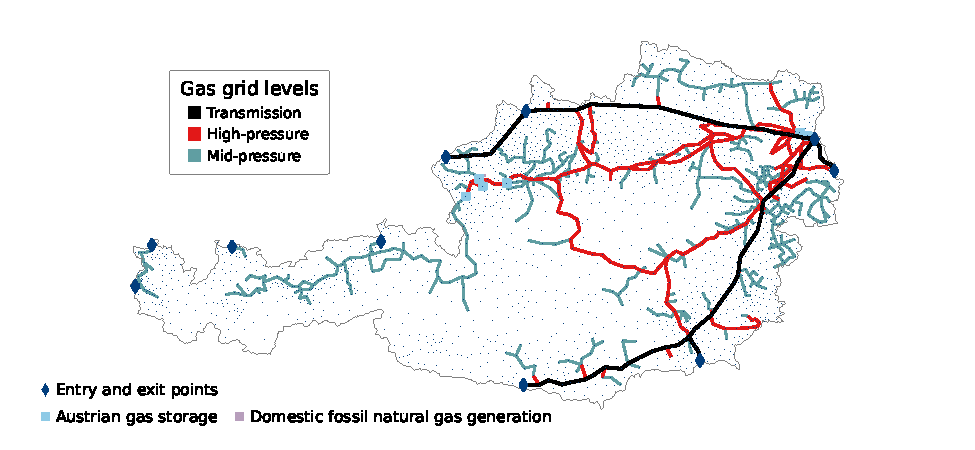
\includegraphics[width=1\linewidth]{figures/method/existing_gas_grid/2023_existing_natural_gas_grid.pdf}
	\caption{Representation of the existing natural gas grid in Austria in the model.}
	\label{method:existing_gas_grid}
\end{figure}

In total, the existing natural gas grid, serving as the starting gas grid, consits of transmission, high-pressure, and mid-pressure pipelines that have in total a length of around \SI{6700}{km}. Below is a brief description of how the authors of the study determined the existing Austrian gas grid in their model as a third party. The fact is that data about gas grids, especially at the distribution grid level, is scarcely accessible to the public. However, data is available for the transmission grid level and for gas storage, for example, published by ENTSO-G \cite{entsog}. At the distribution grid levels, data was partly provided in the form of shapefiles (which is a digital vector storage format for storing geographic location and associated attribute information, such as transport capacities in the context here) upon request (see \cite{zwickl2023design}). Where data on the distribution grid was not available, the location of the high-pressure and mid-pressure pipelines is determined manually (i.e., by comparison with publicly available maps and illustrations from the Austrian energy regulator \cite{econtrol_grid1}) and transport capacities are estimated. This includes the age structure of gas pipelines, for which some information is available on the Internet. The latter can be found, for example, on the websites of the distribution grid operators. The resulting Austrian gas grid, consisting of gas pipelines at the transmission, high-pressure, and mid-pressure grid levels, is then overlaid on the map of Austria at the level of municipalities. There are 2095 Austrian municipalities in total according to the NUTS nomenclature. So those municipalities with natural gas demand and crossing the resulting gas grid are a node in the gas grid graph. As mentioned, there are 657 of such nodes building the existing Austrian gas grid in the model. The connection between two of these nodes are one of the 738 pipeline sections in the model. If a municipality with natural gas demand does not have an intersection with a gas pipeline of the existing grid (e.g., because only a low-pressure pipeline connects is available, which is not considered in the existing gas grid), the demand (and/or generation) is assigned to the nearest node with the shortest distance. 

\subsection{Scenarios}\label{scenarios}
In the absence of a holistic modeling view of the energy system across all energy sectors and sources in this study, the scenarios are of particular importance. In a precise level of energy source use that is modeled in an optimal way in these holistic modeling approaches, the scenarios and their underlying narrative define the degree of electrification, or the use of renewable natural gas and hydrogen in the process of decarbonizing the energy system when replacing fossil natural gas. Based on the degree of electrification, natural gas and hydrogen, this study here does not guarantee, as it is also not the focus, optimality regarding the use of the different energy carriers in a decarbonized Austrian energy system, with the scenarios providing estimates particularly for the development of the amounts of natural gas demand and generation (incl. import and export from and to neighboring countries). The scope is much more on: if we have these amounts and localization of natural gas demand and generation in Austria given, which gas grid is required for balancing both.\vspace{0.3cm}

With this in mind, four different scenarios are defined. They are called "Electrification", "Green Gas", "Decentralized Green Gas" and "Green Methane" and span a wide range of the development of gas demand and generation in Austria. All the four scenarios are based on published national decarbonization scenarios for the Austrian energy system. For example, the scenario Electrification is based on the 2023 \textit{Transition Szenario}, recently fundamentally updated and published by the \textit{Environment Agency Austria} \cite{umweltbundesamt}. Figure \ref{fig:scenario_narratives} gives a characterization of the four scenarios by in total eight dimensions, allowing a qualitiative comparison regarding natural gas demand, generation and its spatial concentration. Based on this qualitative overview of the four scenarios, the natural gas demand is the lowest in the scenario Electrification (Elec) with \SI{7.2}{TWh}, and the highest natural gas demand is in the scenario Green Methane (GM) with \SI{84.2}{TWh}, where we see in Table \ref{tab:scenario_demand} and \ref{tab:scenario_generation} the quantitative numbers of natural gas demand and domestic generation in the four scenarios in 2040, respectively. Latter, for instance, accounts for \SI{91.9}{\%} of the natural gas demand in Austria 2022. 

\definecolor{Gray}{gray}{0.95}
\begin{table}[h]
	\centering
	\setlength{\extrarowheight}{1em}
	\resizebox{1\textwidth}{!}{
		\begin{tabular}{lrrrr}
			\toprule
			Scenario & Elec & GG & DGG & GM\\\hline
			Natural gas demand in 2030&\SI{49.8}{TWh}&\SI{60.3}{TWh}&\SI{63.4}{TWh}&\SI{79.4}{TWh}\\
			\textcolor{white}{Natural gas demand} in 2040&\cellcolor{Gray}\SI{7.2}{TWh}&\cellcolor{Gray}\SI{9.5}{TWh}&\cellcolor{Gray}\SI{20.3}{TWh}&\cellcolor{Gray}\SI{84.2}{TWh}\\\hline
			2040's share of 2022's demand&\SI{9.0}{\%}&\SI{11.0}{\%}&\SI{23.5}{\%}&\SI{91.9}{\%}\\\hline
			Reference for the demand&\cite{umweltbundesamt}&\cite{Energieagentur}&\cite{Energieagentur}&\cite{Energieagentur}\\
			\bottomrule
	\end{tabular}}
	\caption{Natural gas demand in Austria the four scenarios in 2030 and 2040 and comparison with the demand in 2022. Values taken and build on decarbonization scenarios developed and published by the \textit{Environment Agency Austria} \cite{umweltbundesamt} and \textit{Austrian Energy Agency} \cite{Energieagentur}. Abbreviations: Electrification (Elec), Green Gases (GG), Decentralized Green Gases (DGG), Green Methane (GM).}
	\label{tab:scenario_demand}
\end{table}

For the interpretation of the study results, three aspects in the scenario definition are crucial. Therefore, they are highlighted here in particular: 

\begin{itemize}
	\item By the target year 2040, only renewable gases are used to supply Austria's natural gas demand in all the four scenarios. This applies to both the domestic generation (i.e., biomethane based on biogas and synthetic natural gas based on renewable energy) and to the imports of natural gas.
	\item In three of the four scenarios (Electrification, Green and Decentralized Green Gases), the renewable domestic natural gas generation supplies the complete demand. As a consequence, there is a national balance between generation and demand in Austria 2040 and no imports are needed. 
	\item In these three chosen scenarios, the transmission grid only transports gas across Austria and is not used to meet demand in Austria, as, where no imports are needed, the transmission and distribution grids are physically and economically separate. The separation of the two grids is reflected in the results in that the costs of the transmission grid are borne by Austrian consumers only when imports are needed. This is only the case in the GM scenario.\footnote{Whether or not the physical separation of the transmission and distribution grids in such case where there is no need for imports is reasonable for energy security reasons is beyond the scope of this paper.}
\end{itemize}

\begin{table}[h]
	\centering
	\setlength{\extrarowheight}{1em}
	\resizebox{1\textwidth}{!}{
		\begin{tabular}{lrrrr}
			\toprule
			Scenario & Elec & GG & DGG & GM\\\hline
			Natural gas generation in 2030&\SI{4.0}{TWh}&\SI{5.0}{TWh}&\SI{5.0}{TWh}&\SI{5.0}{TWh}\\
			\cellcolor{white}\textcolor{white}{Natural gas generation} in 2040&\cellcolor{Gray}\SI{7.2}{TWh}&\cellcolor{Gray}\SI{9.5}{TWh}&\cellcolor{Gray}\SI{20.3}{TWh}&\cellcolor{Gray}\SI{30.2}{TWh}\\\hline
			2040's share of biomethane&\SI{7.2}{TWh}&\SI{9.5}{TWh}&\SI{9.5}{TWh}&\SI{9.5}{TWh}\\
			2040's share of synthetic gas&\SI{0}{TWh}&\SI{0}{TWh}&\SI{10.7}{TWh}&\SI{20.6}{TWh}\\
			2040's share of fossil gas&\SI{0}{TWh}&\SI{0}{TWh}&\SI{0}{TWh}&\SI{0}{TWh}\\\hline
			2040's share of the demand&\SI{100}{\%}&\SI{100}{\%}&\SI{100}{\%}&\SI{35.9}{\%}\\\hline
			Reference for the generation&\cite{umweltbundesamt}&\cite{Energieagentur}&\cite{Energieagentur}&\cite{Energieagentur}\\
			\bottomrule
	\end{tabular}}
	\caption{Domestic renewable natural gas generation in Austria 2030 and 2040. Three of the four scenarios consider a complete supply of the national natural gas demand by renewable domestic generation. Values taken and build on decarbonization scenarios developed and published by the \textit{Environment Agency Austria} \cite{umweltbundesamt} and \textit{Austrian Energy Agency} \cite{Energieagentur}. Abbreviations: Electrification (Elec), Green Gases (GG), Decentralized Green Gases (DGG), Green Methane (GM).}
	\label{tab:scenario_generation}
\end{table}

Finally, three aspects should be pointed out. Visualizations of the domestic gas generation and demand are given in \ref{app:visualization}. Those maps combined with the qualitative overview of the scenarios given in Figure \ref{fig:scenario_narratives} should sufficiently explain the scenarios for this paper's aim. Whereas the transit of natural gas through Austria is taken from existing modeling studies \cite{frontier2020, frontier2023}, regarding the transit of natural gas, except for the scenario Green Methane (GM), it is assumed that the domestic generation covers the national demand in 2040. In addition, the repurposing of existing gas pipelines for hydrogen transport is also taken from existing studies published by the Austrian gas grid operator \cite{aggm_agid}. 

\afterpage{\clearpage}
\begin{sidewaysfigure}[h]
	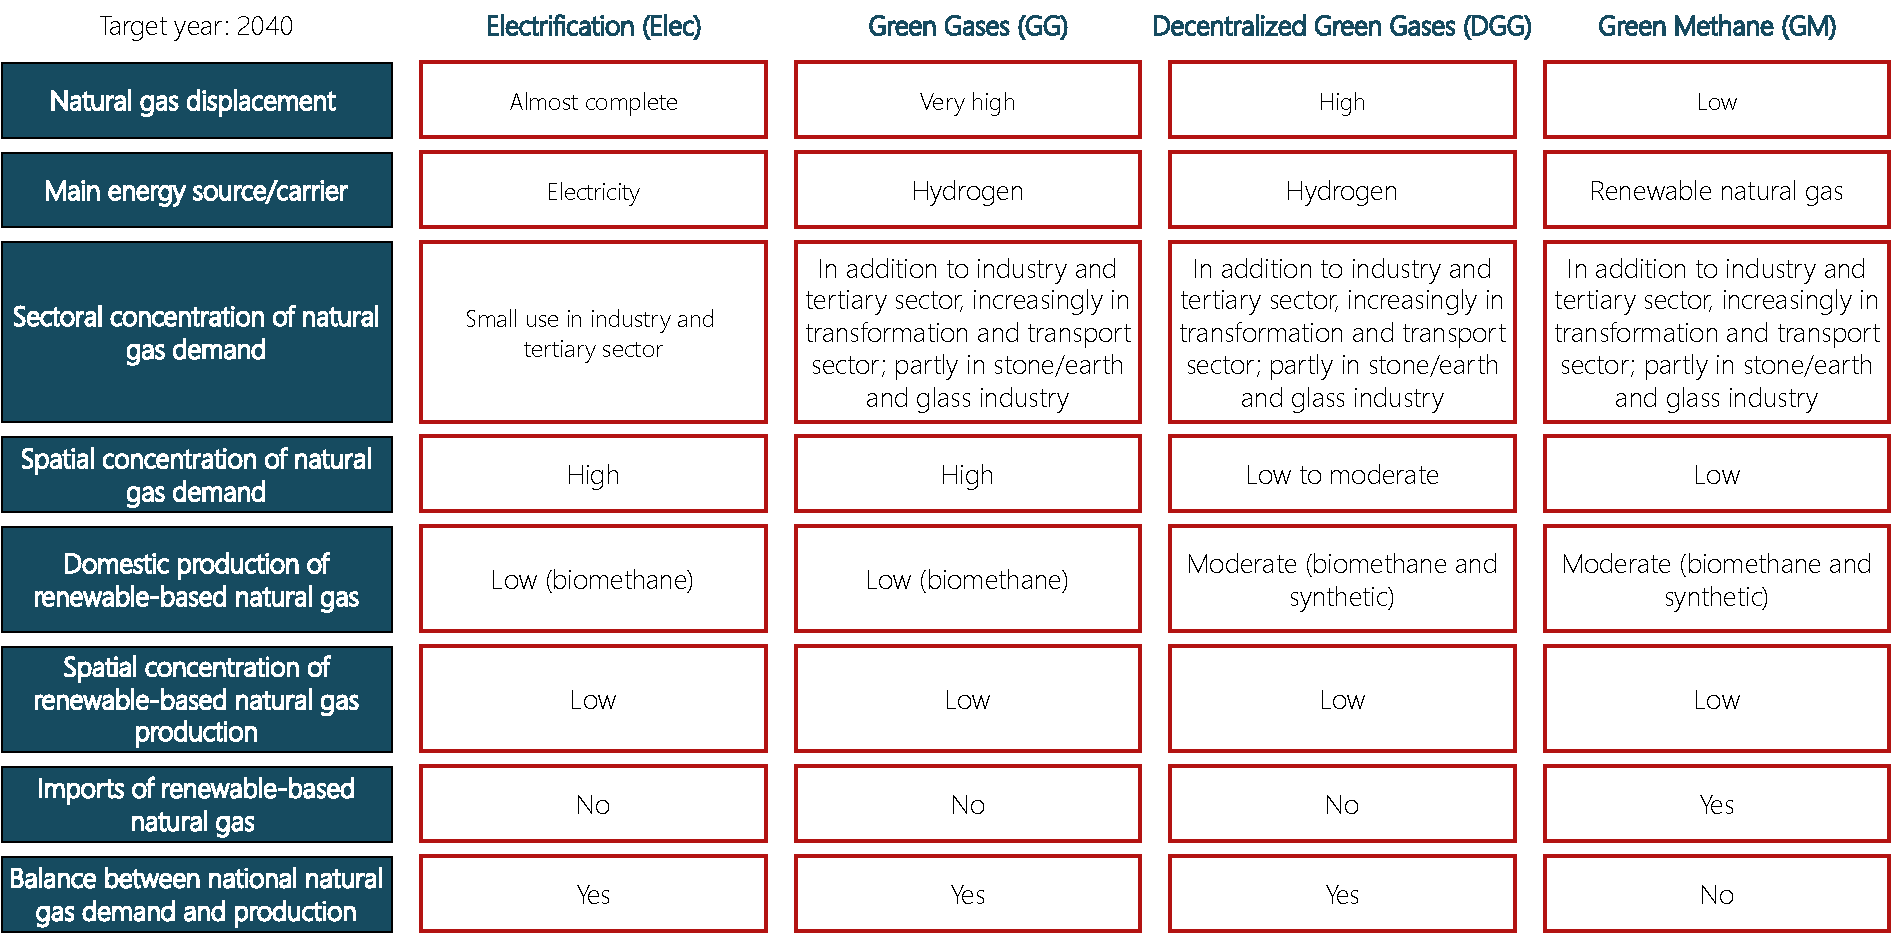
\includegraphics[width=1\linewidth]{figures/method/scenario_narrative.pdf}
	\caption{Overview of the most relevant dimensions characterizing the four scenarios. Storylines and narratives of the scenarios build on decarbonization scenarios developed and published by the \textit{Environment Agency Austria} \cite{umweltbundesamt} and \textit{Austrian Energy Agency} \cite{Energieagentur}.}
	\label{fig:scenario_narratives}
\end{sidewaysfigure} 
